\section{Biological Background}

\begin{figure}[h]
  \centering
	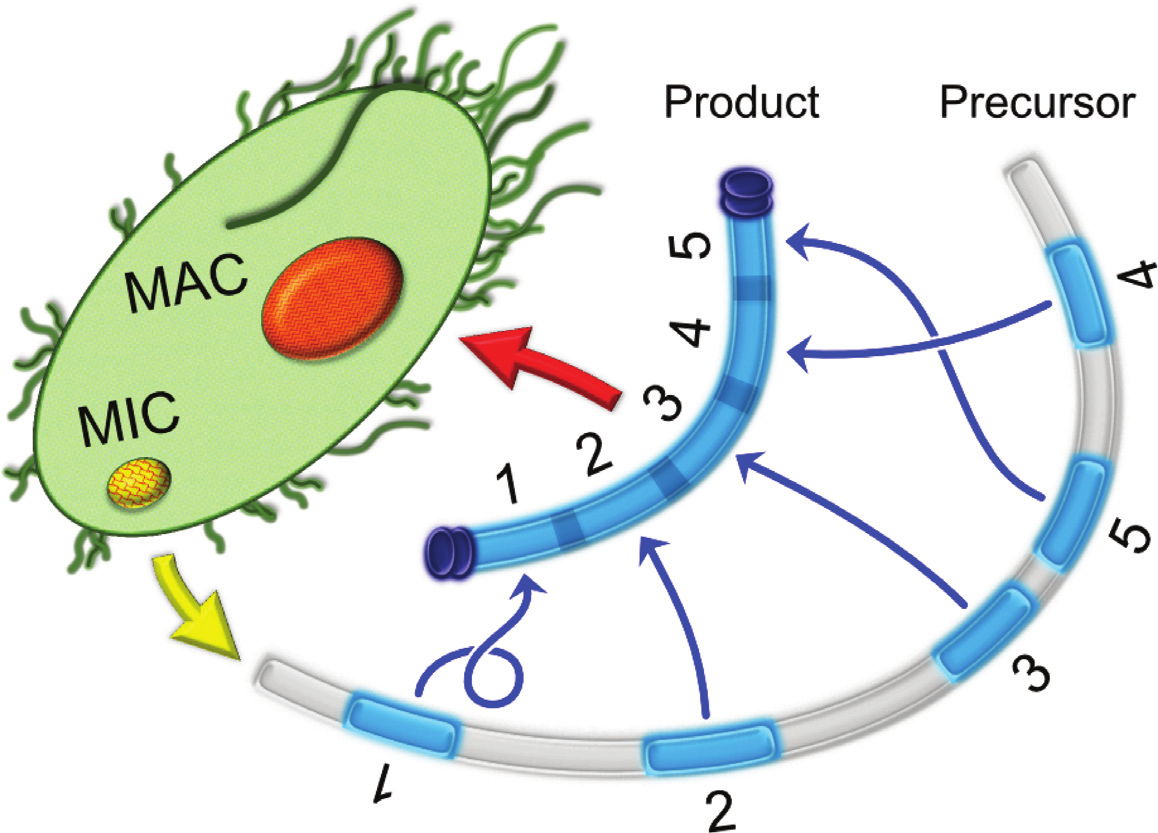
\includegraphics[width=250px]{0}
  \caption{In the somatic macronucleus (MAC), chromosomes assemble from precursor MDS building blocks (blue), which may be scrambled in some species. In the germline micronucleus (MIC), the Macronuclear Destined Sequences (MDSs) for all somatic chromosomes are dispersed over the long chromosome, and interrupted by Internally-Eliminated Sequences (IESs) and other noncoding DNA (gray). In some cases, an MDS may appear in a permuted order, or inverted\cite{mdsiesdb}.
}
\end{figure}

Ciliated protists (microbial eukaryotes using cilia for locomotion) exhibit nuclear dimorphism through the presence of separate germline and somatic nuclei. The somatic macronucleus (MAC) provides templates for the transcription of all genes required for asexual growth while the germline micronucleus (MIC) is used for the exchange of meiotic products during sexual reproduction \cite{mdsiesdb}. The MAC DNA is the one actively expressed and effectively results in the phenotype of the organism.

Several species of ciliates, such as \textit{Stylonychia} or \textit{Oxytricha}, go through extensive gene rearrangement while differentiating somatic macronuclei from germline micronuclei. This process entails an extensive fragmentation, elimination and sometimes broader rearrangement of the germline DNA, coupled to DNA amplification and telomere addition \cite{ciliatedDNA} and form the somatic macronuclei, all under the epigenetic control of novel non-coding RNA pathways \cite{programmedgenome}. The extent and the nature of these operations varies among ciliate species.

Each gene in the macronucleus may be present in the micronucleus as several nonconsecutive segments (macronuclear destined sequences, \textbf{MDSs}) separated by non-coding DNA. During macronuclear differentiation, the non-coding fragments (internal eliminated sequences, \textbf{IESs}) that interrupt MDSs in the micronucleus are deleted. Moreover, the order of the MDSs in the micronucleus may not be consecutive, in which case formation of the macronucleus requires unscrambling of the MDS order, as well as IES removal. There exist \textbf{pointer}-like sequences that are repeated at the end of the \textit{n}th MDS and at the beginning of the \textit{(n + 1)}st MDS in the micronucleus. Each pointer sequence is retained as only one copy in the sequence in the macronucleus \cite{ANGELESKA2007706}.

The general RNA-guided mechanism that regulate and lead this process of assembly is not known, theoretical investigations can be found in \cite{Brijder2007} and \cite{Ehrenfeucht:2004:CLC:971120}.


\section{Biological Motivation}
The guided genome rearrangement problem has (and it's) been extensively \cite{Ehrenfeucht:2004:CLC:971120} studied, both as biochemical process and mathematical model, as it provides an exaggerated case of a phenomenon observed among different species in different ways \cite{ANGELESKA20093020}. Similar broad scale, somatic rearrangement events occur in many eukaryotic cells and tumors.

Many discrete and topological models, mathematical approaches, biological and biochemical explanations and speculations on the theme can be found in literature (such as \cite{prescott2001} \cite{Brijder2014} \cite{ANGELESKA2007706} and \cite{programmedgenome}).

\section{Formalisation}

\begin{figure}[h]
  \centering
    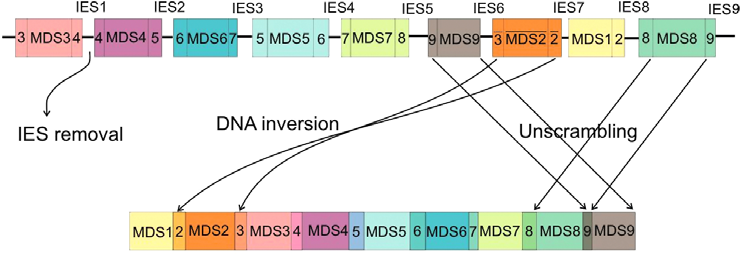
\includegraphics[width=\textwidth]{1}
  \caption{Schematic representation of the scrambled Actin I micronuclear germline gene in Oxytricha nova (top) and the correctly assembled macronuclear gene (bottom). Each block represents an MDS, and each line between blocks is an IES. The numbers at the beginning and at the end of each segment represent the pointer sequences. Note that MDS3-MDS8 require permutation and inversion to assemble into the orthodox, linear order MDS1-MDS9 in the macronucleus. The bars above MDS2 and its pointers indicate that this block is inverted relative to the others, i.e., this sequence is the Watson - Crick reverse complement of the version in the macronucleus; from\cite{prescottgreslin}.}

\end{figure}

The recognised events in the rearrangement process are:

\begin{itemize}
	\item The MAC begins a copy of the MIC DNA. The chromosomes are fragmented and amplified. The result of this process is the \textit{precursor}. $\sim$90\% of the complexity is lost.
	\begin{itemize}
    	\item Fragmentation
    	\item Amplification
    \end{itemize}

	\item From the precursor the final MAC DNA is produced through these further operations:
	\begin{itemize}
    	\item Elimination
    	\item Inversion
    	\item Gene Scrambling - Unscrambling
    	\item Telomere Addition
    \end{itemize}

\end{itemize}

We focus on the second phase, trying to map the following "building blocks":

\begin{itemize}
	\item \textbf{MDSs}, the contiguous sequences copied, inverted or (order) scrambled in the MAC;
	\item \textbf{IESs}, sections not present in the MAC;
	\item \textbf{Pointers}, overlap sections between MDSs in the MAC (maybe inverted), present in multiple copies in the MIC;
\end{itemize}

The "inverse", "reverse", "reverse complement" terms refer to the \textit{Watson-Crick reverse complement} of the sequence.

The goal is to produce a \textit{rearrangement map}: a set of disjoint substrings representing the building blocks, eventual operations they will go through the process (scrambling, inversion) and their "destination" on the produced genome.

\subsection{Real Instance}

Ideally, we want to reach an approach capable of treating the entire MAC and MIC sequenced genomes of \textit{Oxytricha trifallax} or \textit{Tetrahymena thermophila}, available publicy \href{http://oxytricha.princeton.edu/mds_ies_db/}{online} in the \textsc{mds\_ies\_db} ("A database of macronuclear and micronuclear genes in spirotrichous ciliates" \cite{mdsiesdb}).

\textit{Oxytricha trifallax} has a 487.14 M long MIC sequence, rearranging in a 71.47 M characters long MAC \cite{mdsiesdb}.

Formally, given an initial genome(MIC or MAC precursor) and a rearranged one (MAC) the program produces an annotation map of the process the input has been through.

\section{Existent Approaches}

\paragraph{mds-ies-db}\cite{mdsiesdb} proposes an annotation map, presuming the MDSs general pattern (using regular expressions) and using the Basic Local Alignment Search Tool (BLAST \cite{boratyn2013blast}) to flag matching regions.

The algorithm is the following:

\begin{enumerate}
  \item Use provided regular expression to mask macronuclear telomeric sequences.
  \item Blast MAC sequences against MIC sequences.
  \item Process obtained high scoring pairs list resolving overlaps to obtain initial MDS annotation.
  \item Blast MAC sequences against MIC sequences again.
  \item Use obtained high scoring pairs to fill gaps in the initial MDS annotation and get final MDS annotation for MAC.
  \item Output final MDS/IES annotation for MAC and MIC.
\end{enumerate}

An example regular expression used in step \textbf{1} is \texttt{A{0,4}(CCCCAAAA)+C{0,4}}.

During step \textbf{2}, long (at least 28 nucletides) high scoring pairs (HSPs) are found using BLAST. Next, in step \textbf{3} overlapping HSPs are merged (if they overlap at least 50\%).
Step \textbf{4} makes sure that no portion of the MAC sequnces remains uncovered, using BLAST with lower requirements (at least 12 nucletides) that can potentially fill the gaps.
Finally, MIC sub-sequences that are in between HSPs are considered IESs.

\paragraph{}
The recent \textbf{Sorting by Reversals and the Theory of 4-Regular Graphs} \cite{DBLP:journals/corr/Brijder17} shows an interesting approach in describing the \textit{Reversal} evolutionary event and illustrates its correlation to the DNA recombination problem found in ciliates. The \textit{reversal distance} is defined as the least number of reversals required to accomplish the transformation (an efficient algorithm to compute this distance can be found in \cite{Hannenhalli}). The reversal event is then cast as a special case of double-cut-and-join (DCJ) operation (which can happen within a chromosome or between more of them). Similarly, a formula to compute the DCJ distance is given in \cite{Bergeron2006}.

The problem of computing the distance between two permutations is often recast as the problem of computing $d(\pi)$, the reversal distance between a permutation $\pi$ and the identity permutation $(1 2 ... n)$. The reconstruction of one possible sequence of reversals that realizes $d(\pi)$ is called the \textit{sorting by reversals} problem.

The gene assembly in ciliates is finally casted with the theory of sorting by reversals (although ignoring overlap sections).

How 4-regular multigraphs, circle graphs and delta-matroids can be used to study gene assembly in ciliates it's further discussed in \cite{Brijder2014}.

\paragraph{}
\textbf{DNA Recombination through Assembly Graph}\cite{ANGELESKA20093020} takes a more elaborate combinatorial approach, introducing the notion of \textit{assembly graph} as a finite connected graph where all vertices are rigid vertices of valency 1 or 4. The recombination process is then modeled using polygonal paths, tranverse paths and smoothings.